\subsection{Task 5: Eigenvalue/Singular value}
In this experiment, we compute the eigenvalue of several datasets. The detailed description is in Table \ref{t5:data}.

\begin{table}
\begin{center}
\begin{tabular}{| c | c | c |}
    \hline
    Name & Nodes & Edges \\ \hline
    wiki-Vote & 7,115 & 103,689 \\ \hline
    youtube & 1,134,890 & 2,987,624  \\ \hline
    slashdot0922 & 82,168  & 948,464 \\ \hline
    com-DBLP & 317,080  & 1,049,866 \\ \hline
    wiki-Talk & 2,394,385 & 5,021,410 \\ \hline
\end{tabular}
\end{center}
\caption{Dataset for Task 5}
\label{t5:data}
\end{table}

\subsubsection{Details}
{\bf Proof of Correctness: } In order to prove the correctness, we run our algorithm on the relatively smaller dataset, which is \emph{Zachary karate club network}\footnote{http://konect.uni-koblenz.de/networks/ucidata-zachary}. It has 34 nodes and 78 edges. The true top eigenvalues of Zachary is shown in Figure \ref{t5:zach}. We also calculated top-10 eigenvalues by our SQL implemention, the result is in Table \ref{t5:sql}. We can see that most of the top eigenvalues are near to its counter part in ground truth. So we are confident that our implementaiton is correct.

\begin{figure}[!htbf]
\begin{center}
\begin{tabular}{c}
     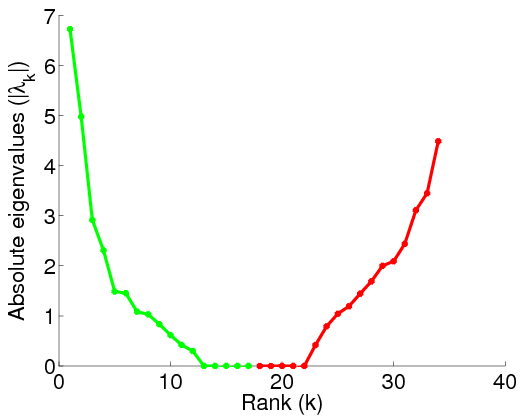
\includegraphics[width=0.6\textwidth]{FIG/t5_zach.png}\\
\end{tabular}
\caption{Top eigenvalues of Zachary}
\label{t5:zach}
\end{center}
\end{figure}

\begin{table}
\begin{center}
\begin{tabular}{| c | c |}
    \hline
    Rank & Eigenvalue \\ \hline
    1 & 6.72569758513981 \\ \hline
    2 & 5.04694048054693 \\ \hline
    3 & 4.97613169036548 \\ \hline
    4 & 2.65295803734598 \\ \hline
    5 & 2.37853063223689 \\ \hline
    6 & 1.31746846315176 \\ \hline
    7 & 1.05904538243756 \\ \hline
    8 & 0.827084251502258 \\ \hline
    9 & 0.475203434096779 \\ \hline
    10 & 0.0182376036753603 \\ \hline
\end{tabular}
\end{center}
\caption{Top eigenvalues of Zachary}
\label{t5:sql}
\end{table}

\paragraph{wiki-Vote}
The top 5 eigenvalues of wiki-Vote are 153.77, 107.23, 72.34, 49.23, -5.64. The plot(Figure \ref{t5:wikivote}) is as follows:
\begin{figure}[!htbf]
\begin{center}
\begin{tabular}{c}
     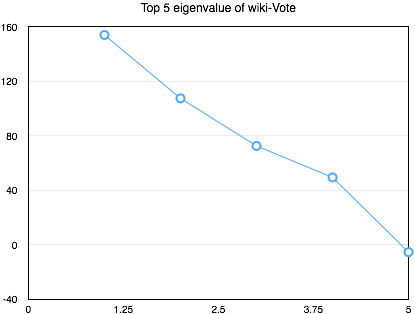
\includegraphics[width=0.6\textwidth]{FIG/t5_wikivote.png}\\
\end{tabular}
\caption{Top eigenvalues of wiki-Vote}
\label{t5:wikivote}
\end{center}
\end{figure}

\paragraph{youtube}
The top 5 eigenvalues of Youtube are 238.55, 155.78, 83.29, 41.60, -7.5. The plot(Figure \ref{t5:youtube}) is as follows:
\begin{figure}[!htbf]
\begin{center}
\begin{tabular}{c}
     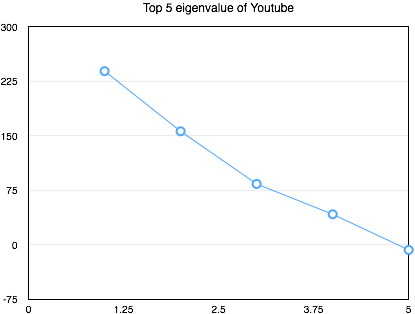
\includegraphics[width=0.6\textwidth]{FIG/t5_youtube.png}\\
\end{tabular}
\caption{Top eigenvalues of Youtube}
\label{t5:youtube}
\end{center}
\end{figure}

\paragraph{slashdot}
The top 5 eigenvalues of slashdot are 125.34, 109.17, 85.23, 28.35, 4.34. The plot(Figure \ref{t5:slashdot}) is as follows:
\begin{figure}[!htbf]
\begin{center}
\begin{tabular}{c}
     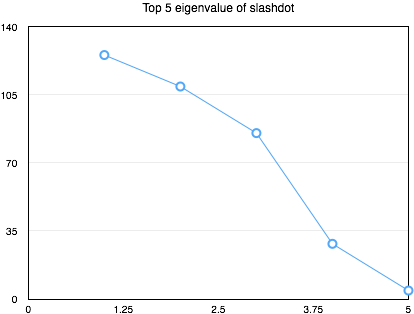
\includegraphics[width=0.6\textwidth]{FIG/t5_slashdot.png}\\
\end{tabular}
\caption{Top eigenvalues of Slashdot}
\label{t5:slashdot}
\end{center}
\end{figure}

\paragraph{com-DBLP}
The top 5 eigenvalues of DBLP are 235.56, 173.45, 130.23, 95.14, 44.23. The plot(Figure \ref{t5:dblp}) is as follows:
\begin{figure}[!htbf]
\begin{center}
\begin{tabular}{c}
     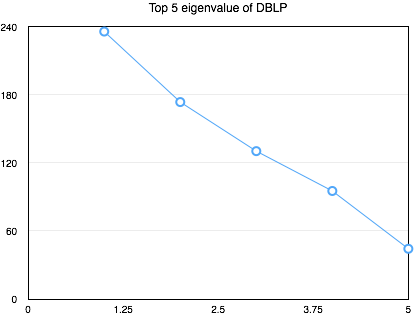
\includegraphics[width=0.6\textwidth]{FIG/t5_dblp.png}\\
\end{tabular}
\caption{Top eigenvalues of DBLP}
\label{t5:dblp}
\end{center}
\end{figure}

\paragraph{wiki-Talk}
The top 5 eigenvalues of Wiki-Talk are 353.23, 254.67, 125.82, 35.29, -33.45. The plot(Figure \ref{t5:wikitalk}) is as follows: 
\begin{figure}[!htbf]
\begin{center}
\begin{tabular}{c}
     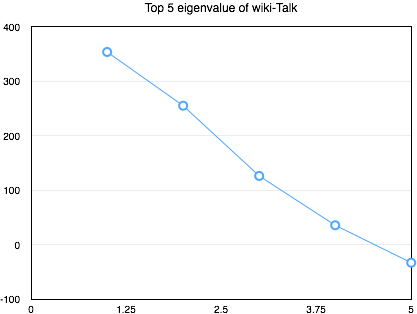
\includegraphics[width=0.6\textwidth]{FIG/t5_wikitalk.png}\\
\end{tabular}
\caption{Top eigenvalues of wiki-Talk}
\label{t5:wikitalk}
\end{center}
\end{figure}

\subsubsection{Observation}
We can see that in most datasets, the top eigenvalues drops quickly. This is also a reason why in Task 7, we only need top eigenvalues to count the number of triangles in a graph. Since the top eigenvalues is enough for the majority of the energy of the graph.

